\newif\ifimagen\imagentrue
\documentclass[11pt]{article}
\usepackage[utf8]{inputenc}\usepackage[top=0.8in, left=1in, right=1in, bottom=0.8in]{geometry}\usepackage[parfill]{parskip}\usepackage{fancyhdr}\usepackage{sectsty}\usepackage[font=small,labelfont=bf,textfont=it]{caption}\usepackage{graphicx}\usepackage{booktabs}\usepackage{array}\usepackage{paralist}\usepackage{verbatim}\usepackage{subfig}\usepackage{mathtools}\usepackage{amssymb}\usepackage{verbatim}\usepackage{listings}\usepackage{color}\usepackage{overpic}\usepackage{enumitem}\usepackage{cite}\usepackage[unicode=true,
    bookmarks=true,bookmarksnumbered=true,bookmarksopen=true,
    bookmarksopenlevel=2, breaklinks=false,pdfborder={0 0 0},backref=false,
    colorlinks=false]{hyperref}\usepackage[svgnames]{xcolor}\usepackage{tikz}\usepackage{tikz}\newcommand{\inputTikZ}[1]{%
        \input{#1}%
    }
\newcommand{\executeiffilenewer}[3]{%
    \ifnum\pdfstrcmp{\pdffilemoddate{#1}}%
        {\pdffilemoddate{#2}}>0%
        {\immediate\write18{#3}}
    \fi
}
\newcommand{\includesvg}[1]{%
    \executeiffilenewer{#1.svg}{#1.pdf}%
    {inkscape -z -D --file=#1.svg --export-pdf=#1.pdf --export-latex}%
    \input{#1.pdf_tex}%
}
\renewcommand{\d}{\,\mathrm{d}}
\newcommand{\dx}[2]{\frac{\textrm{d} #1}{\textrm{d} #2}}
\newcommand{\dd}[2]{\frac{\textrm{d}^2 #1}{\textrm{d} #2^2}}
\newcommand{\pd}[2]{\frac{\partial #1}{\partial #2}}
\newcommand{\pdd}[2]{\frac{\partial^2 #1}{\partial #2^2}}
\newcommand{\e}[1]{\text{e}^{#1}}
\newcommand{\code}[1]{\texttt{#1}}
\newcommand{\inter}[1]{\shortintertext{#1}}
\newcommand{\under}[1]{\underline{#1}}
\let\vaccent\v                                                                 
\newcommand{\uv}[1]{\ensuremath{\hat{#1}}}
\newcommand{\abs}[1]{\left| #1 \right|}
\newcommand{\avg}[1]{\left< #1 \right>}
\let\underdot\d                                                                
\newcommand{\ket}[1]{\left| #1 \right>}
\newcommand{\bra}[1]{\left< #1 \right|}
\newcommand{\braket}[2]{\left< #1 \vphantom{#2} \right|
    \left. #2 \vphantom{#1} \right>}
\newcommand{\matrixel}[3]{\left< #1 \vphantom{#2#3} \right|
    #2 \left| #3 \vphantom{#1#2} \right>}
\newcommand{\grad}[1]{\nabla #1}
\let\divsymb\div                                                               
\renewcommand{\div}[1]{\nabla \cdot #1}
\newcommand{\curl}[1]{\nabla \times #1}
\let\baraccent\=                                                               
\renewcommand{\=}[1]{\stackrel{#1}{=}}

\pagestyle{empty}
\thispagestyle{empty}
\begin{document}
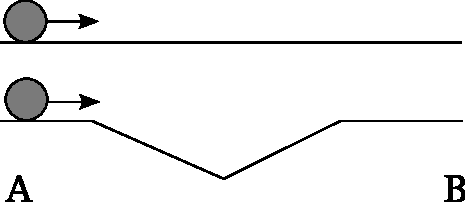
\includegraphics[width=0.3\textwidth]{./rolling_balls.pdf}
\clearpage% page: 0
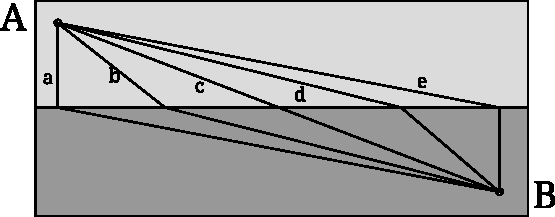
\includegraphics[width=0.6\textwidth]{./runners.pdf}
\clearpage% page: 1
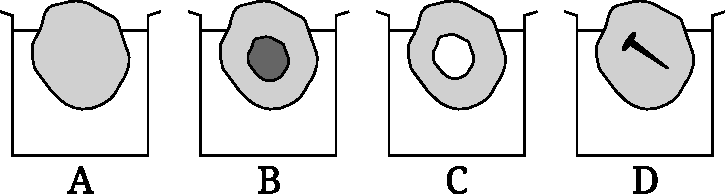
\includegraphics[width=0.8\textwidth]{./vessels.pdf}
\clearpage% page: 2
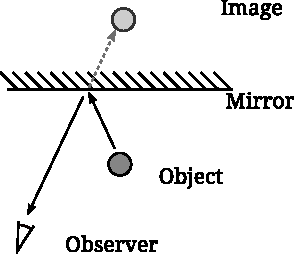
\includegraphics[width=0.3\textwidth]{./mirrors_question_diag.pdf}
\clearpage% page: 3
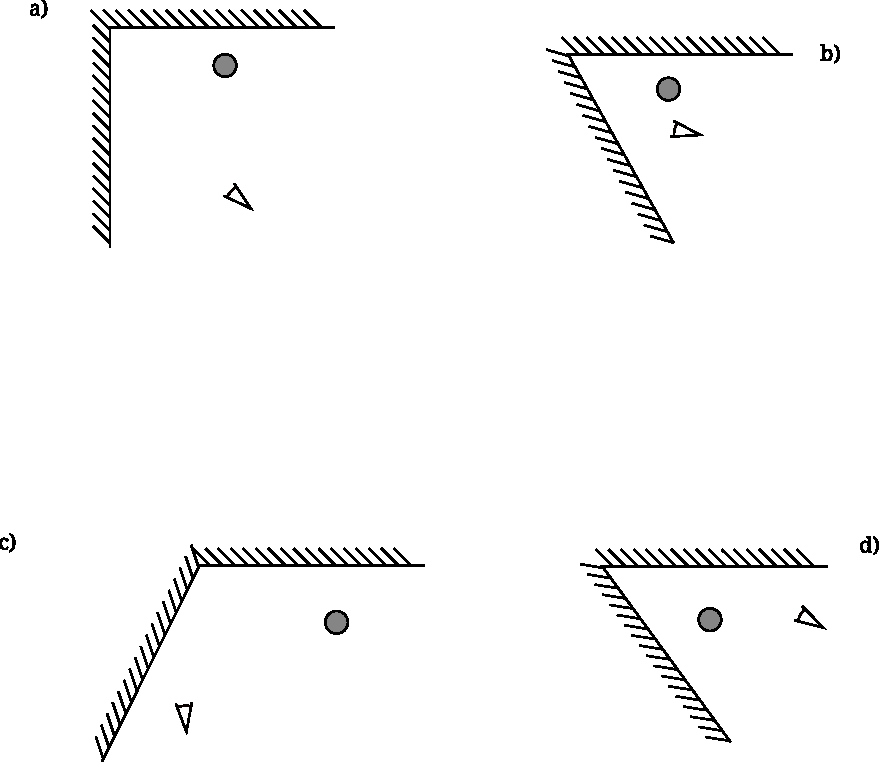
\includegraphics[width=0.9\textwidth]{./mirrors_question.pdf}
\clearpage% page: 4
\renewcommand{\@maketitle}{
\newpage
 \null
 \vskip 2em%
 \begin{center}%
  {\Large \@title \par}%
 \end{center}%
 \par}
\setcounter{section}{0}
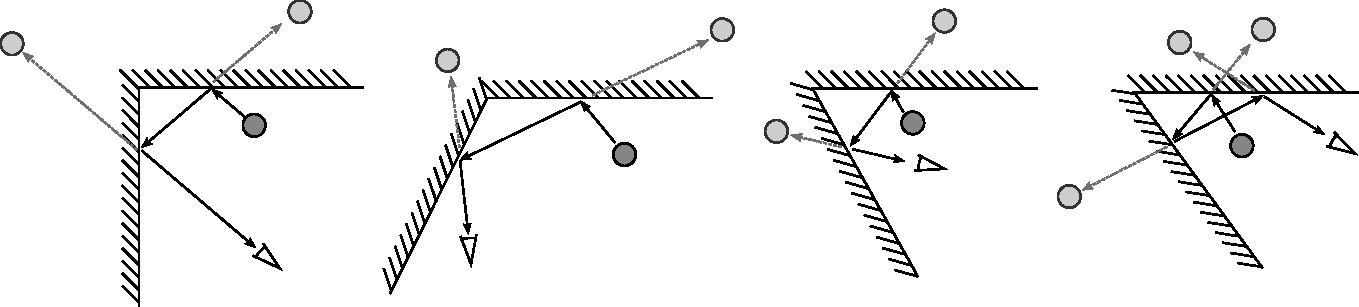
\includegraphics[width=1.0\textwidth]{./mirrors_answer.pdf}
\clearpage% page: 5
%Options: 
\end{document}
